Nous avons choisi de nous demander si il existe un lien entre le
nombre de warnings de chaque type renvoyés pendant la compilation et la
qualité de la gestion mémoire attribuée par valgrind.

Nous pour cela séparé notre jeu de données en deux: les programmes
ayant une gestion mémoire décrite comme clean par valgrind, et les
autres.
Nous avons ensuite effectué trois tests de Mann Whitney, un pour chaque
type de warning (Clang, MinorWarning de gcc, MajorWarning de gcc),
avec pour hypothèse nulle ``Il n'y a pas de différence significative
du nombre de warnings à la compilation entre les programmes en fonction
de la qualité de leur gestion mémoire.''.

Pour les Major Warning, la p-value retournée par le test est de
0.02165, au risque d'erreur 5\%, nous pouvons donc rejeter
l'hypothèse nulle. Nous en concluons que le nombre de warnings majeur gcc
est supérieur pour les programmes ayant une gestion mémoire non propre
(figure \ref{fig:MW_valgr}).

\begin{figure}[h]
  \centering
  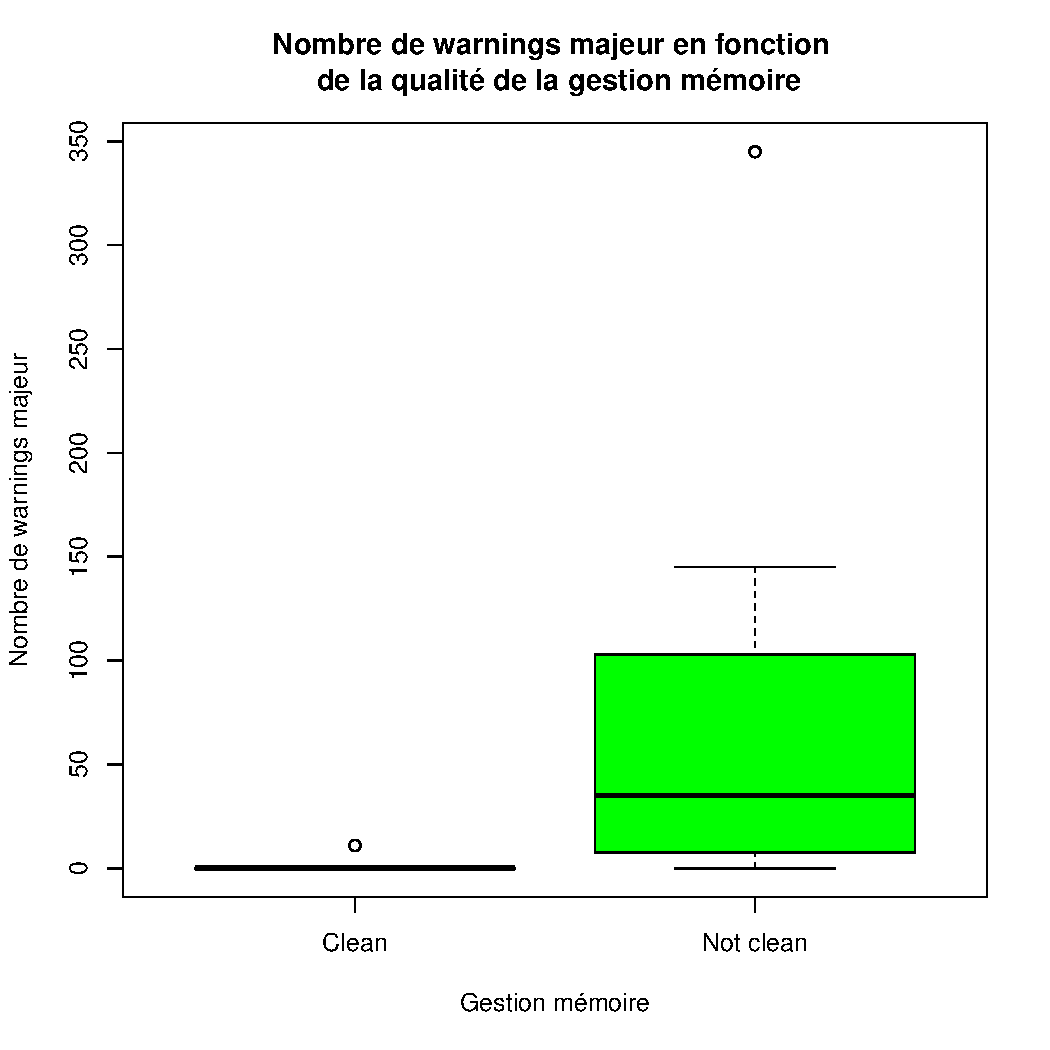
\includegraphics[width=.48\textwidth]{figures/MW_valgr.pdf}
  \caption{}\label{fig:MW_valgr}
\end{figure}

Pour les Warning mineurs et Clang respectivement, la p-value retournée
par le test est de 0.1645 et 0.7348. Au risque d'erreur 5\%, nous ne
pouvons donc pas rejeter l'hypothèse nulle. Nous en concluons que le
nombre de warning mineur gcc et clang n'est pas sensiblement inférieur
pour les programmes propres.
